\documentclass{article}
\usepackage{natbib, graphicx}
\begin{document}
\title{Illuminating poverty: Using satellite light detection for a poverty indicator}
\maketitle
\begin{abstract}
Satellite data includes areas that are difficult to reach via surveys or traditional big
data sources like cash registers and computers. We consider the use of luminosity data
from space as a correlate to poverty, using data from Bangladesh and Guatemala.
\end{abstract}

\section{Introduction}

\citet{chen:pnas} and \citet{henderson:nber} wrote on using luminosity as a measure of GDP. However, GDP and poverty are very imperfectly correlated.

\section{Model and methods}

\subsection{Model}
Consider a set of $N$ agents, each of whom could produce a light source. The odds of
producing a light source are a function of availability of electricity, urbanization, and poverty.

Light intensity is additive: given one source producing $L_1$ candelas of light, and a
second producing $L_2$ candelas, the total luminosity observed is simply $L_1+L_2$.

All this will wind up with a form suitable for regression 

$$L_i = \beta_{l0} + \beta_{l1} Pv + \beta_{l2} El + \beta_{l3} Ur + \epsilon,$$

where $Pv$ is our poverty measure, $El$ is electrification, $Ur$ is urbanization.
We can rewrite this as 

$$Pv = \beta_0 + \beta_1 L_i  + \beta_2 El + \beta_3 Ur + \epsilon,$$

where the relationship between $\beta_{l0}$ and $\beta{0}$, $\beta_{l1}$ and $\beta_1$, \dots, is easily calculated.

\subsection{Data}
We use luminosity data from NOAA. 
Each area consists of a set of pixels covering an upazila; let the pixel count for upazila
$u$ be $P_u$ and a pixel $j$'s intensity be $I_j$.


Below, we will use a few summary metrics for intensity in the region, including $$\mu = \frac{\sum_j I_j}{P_u}$$
and 
$$\ln\mu = \frac{\sum_j \ln(I_j)}{P_u}.$$

The intent of the second measure is based on the assumption that pixel intensity in a
region is lognormally distributed. We found the Kullback-Leibler divergence between a true
lognormal distribution and the histogram of data was good.

\section{Results}
The raw correlation between luminosity and our poverty measure is pretty good


\begin{figure}
\begin{center}
\hrule
\begin{tabular}{lrrrrrrr}
& poverty        &   $\ln\mu$  &    $\Delta\ln\mu$ &  pop density &   \% electric & \% urban \\
poverty        &   1 & -0.351&  -0.352&        -0.111&    -0.544& 0.0467\\
$\ln\mu$       & -0.351&     1  &   0.434&       0.198&    0.840& 0.0413\\
$\Delta\ln\mu$ & -0.352&  0.434&    1 &         0.154&    0.463&0.0687\\
density    & -0.111&  0.198&   0.154&           1 &    0.231& 0.0536\\
\% electric     & -0.544&   0.84&  0.463 &        0.231&      1    &  0.262\\
\% urban       & 0.0467& 0.0413&  0.068&       0.0536&     0.262&     1
\end{tabular}
\hrule
\end{center}
\caption{Correlation coefficients.}
\end{figure}

\begin{figure}
\begin{center}
%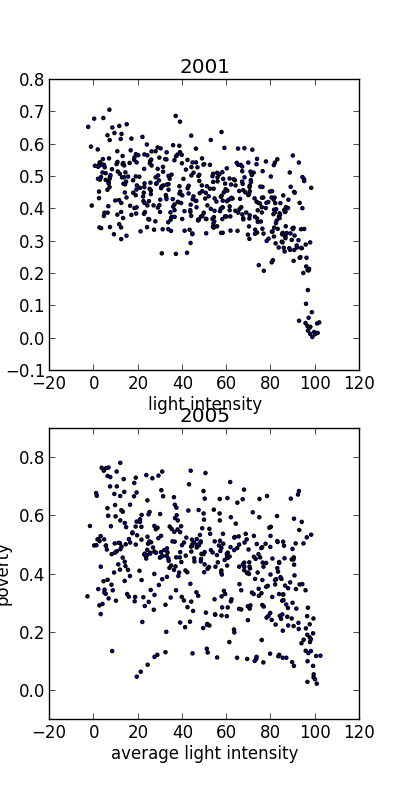
\includegraphics[width=\textwidth*\real{0.8}]{dotplot.png}
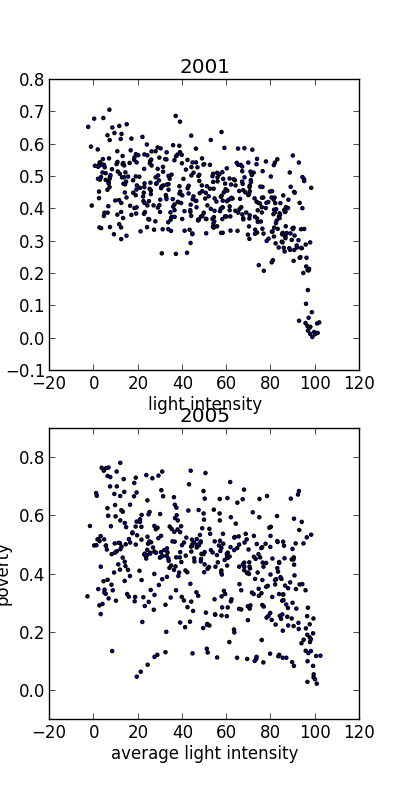
\includegraphics[width=7cm]{dotplot.png}

\end{center}
\caption{Scatterplot of light and poverty.}
\end{figure}

We ran a few regressions, including obvious correlates like percent with access to
electricity and population density, and found that poverty is still well-predicted by
log luminosity, and log luminosity is well-predicted by poverty.

Here are some extremely attractive maps to get the point across.

We then did the predictive exercise, using luminosity measures from 2001--2005 in a
training subset to predict poverty in 2005. We did OK.

\section{Conclusion}


\bibliographystyle{plainnat}
\bibliography{luminosity}

\end{document}
